
\chapter{Approach}\label{chapter:realization}

In this chapter, the main approach of this thesis is presented. The chapter starts with an abstract description of the approach with the aim of providing a high-level overview of the underlying concepts (\autoref{sec:concept}). Then, a list of requirements and desirable quality attributes is given (\autoref{sec:requirements}) on the basis of which the approach is later evaluated (\autoref{chapter:discussion}). The section that follows gives a concrete example of how the system may be realized. For this, an exemplary technology stack is presented, whereby each of the employed technologies is discussed in detail (\autoref{sec:realization}). This part builds the basis for the subsequent chapter, where a system based on the presented technologies is evaluated.

%
%
%
%
%
%
%
%
%
%

\section{Concept} \label{sec:concept}
The objective of this thesis is to explore methods to handle the increased demand for computational power and data collection in mobile cyber-physical systems, and in particular automotive systems. For this, an approach is presented that allows single vehicular functions to be outsourced to the cloud.
Since connectivity in such systems is often unstable, the offloading must be accomplished in an instantaneous and smooth fashion. At the same time, operation may not be interrupted and the cohesion of the system must be preserved at all times. 
%The key concept to facilitate this is replication. 

\subsection{Partitioning of Functionality}
At the core of the approach is the idea to split functionality into isolated units which may be deployed redundantly on both, the vehicle's on-board system, and on high-performance machines in remote data centers. For this, the system needs to facilitate the clean separation of functionality according to responsibilities. The service-oriented architectural paradigm is a suitable way to achieve this\todo{rephrase}. Service-orientated architectures aim to divide functionality into isolated modules, so-called \emph{services}. Each service provides an offering to other services by means of a clearly defined, preferably immutable and machine-readable interface. By guaranteeing that these interfaces rarely change, a formal \emph{service contract} is put in place which ensures continuous interoperability between the services. Examples of service offering may be the provisioning of some sort of data, or functionality (algorithms and business logic). All services of the system are working together in synergy to achieve a common goal, \ie , the continuous operation of a vehicle. 


\subsection{Communication Paradigm}
As mentioned, an inherent challenge distinctive to the domain at hand is the highly unreliable and unpredictable communication channel to the cloud. Remotely deployed services are thus massively ephemeral in their nature. As a consequence, the topology of the service network is constantly changing. This requires the communication method between services to be entirely anonymous. \Ie , services shall not have references to other services as these may be unavailable momentarily. Management of references (addition of new references and invalidation of old ones) is highly ineffective and therefore should be avoided at all costs. A communication paradigm that meets this requirement is the publish-subscribe paradigm. In a publish-subscribe system, services exchange information by means of topics. Services that provide data may push data on a given topic, and services that wish to receive that data may subscribe to that topic. Services do not know where a given data sample came from or which service will receive their data sample. Thus, communication is anonymous.

\todo[inline]{

Switch must be feasible at run-time

transition must be fluent

Communication shall be ubiquitous

A major problem in automotive architectures is the management of data. As a result of the historically grown nature, whereby each ECU is highly specialized in a very narrow range of duties, there is no consistent model of data---each ECU has its own view on data which may very well differ from other ECU's view \cite{broy2006challenges}. It is therefore evident that data need to be put into the center of attention. Data-centricity is a communication style that follows this goal. provides common, consistent view on data. global shared data space.
}

The method of exposition is data-centric: instead of providing \emph{methods} that other services may invoke (RPC style), services offer \emph{data}. Any service interested in receiving a certain kind of data listens in on a topic on which such data is published. This approach greatly helps to decouple the system as services do not need to have references to one another. As a result, services may evolve without having to deal with interface interdependencies.


\subsection{Replication}
The approach aims to achieve superior computing performance by way of horizontal scaling. Replication is therefore key. Thus, the system shall support the fast provisioning of services in the form of \emph{service instances}. The service-oriented approach alleviates replication tremendously, provided that certain design principles are applied. Hence, throughout the design and implementation of the envisioned system, several design goals need to be kept in mind. Firstly, services ought to be \textbf{stateless}. Statelessness facilitates replication as sharing state among many instances proves to be difficult. Consistency is hard to achieve and locking mechanisms may become a bottleneck.\todo{more on consistency models this in tanenbaum...} Furthermore, services should be \textbf{fine-grained}. A high-resolution granularity allows for detailed control over which services should be replicated. That way, computational bottlenecks can be more easily singled-out and eliminated. An added benefit is increased extensibility and faster software updates. However, trade-offs need to be considered. If services are too fine-grained, they need to communicate more, and as a result, the communication channel might become a bottleneck. Furthermore, too many services unnecessarily increase complexity.

Another design goal to keep in mind is \textbf{isolation}. Services should have limited knowledge of both, location and topology. The aim should be to hide anything that isn't directly related to the reception of data. Through that, loose coupling is achieved. One aspect of isolation is self-containment. Services should be kept together with all their dependencies as a single unit that may be deployed on any hardware platform. By packaging services in self-contained environments, they may be moved between different computing nodes. This property is the most important one to achieve cloud scalability. Commonly used tools to facilitate this are virtualization and containerization.

The last question that remains is how services are connected. Since services may be duplicated and migrated between computing nodes, special emphasis needs to be put on location/relocation transparency and dynamic topology management. In the approach, the use of virtual overlay networks is suggested for this purpose. Especially challenging is the fact that the overlay must work on top of a substrate network made up of numerous globally dispersed nodes, of which some continuously change their location. As a result, the substrate network is exceptionally unreliable.

\subsection{Example}

\begin{figure}[htpb]
  \centering
  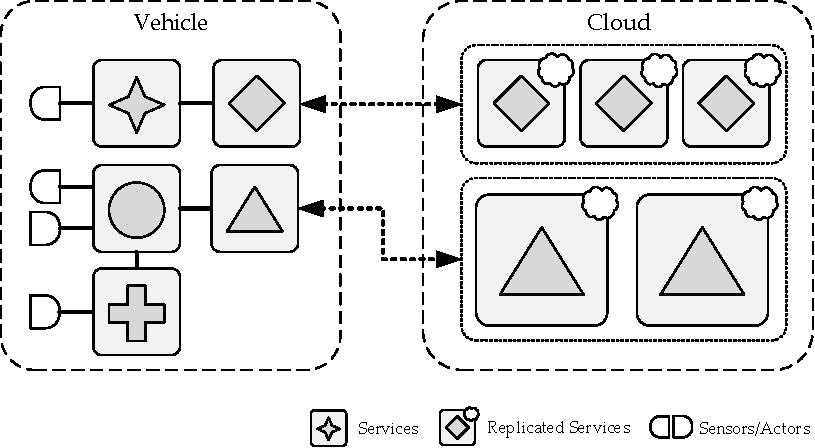
\includegraphics[width=0.8\textwidth]{figures/idea.pdf}
  \caption[Conceptual sketch of the approach]{Conceptual sketch of the approach, demonstrating location transparent replication of services in the cloud}\label{fig:idea} \todo[inline]{add cloud exclusive service?}
\end{figure}

\autoref{fig:idea} depicts a schematic example. The box on the left-hand side represents a vehicle. In the vehicle, several interconnected services are deployed. What is omitted from the image is that these services run on distributed embedded devices spread over the vehicle's on-board system. Several of these services rely on sensor data and/or control actors (indicated by the semicircles). On the right-hand side, the cloud is depicted, which, in actuality, is a collection of high-performance computing nodes. Vehicle and cloud are physically separated and connected via some sort of network, which the vehicle may access by means of a cellular network. As can be observed in the figure, some of the vehicle-intrinsic services are replicated in the cloud (\ding{117}, \ding{115}). Examples of such services could be functions for predicting trajectories, gaze detection, or machine learning algorithms. The duplication and varying size of the service boxes depicted in the image is indicative of horizontal and vertical scaling, respectively. It doesn't always make sense to replicate services in the cloud, \eg , because they are computationally inexpensive, or because they require access to sensors and actors which are inherently bound to the vehicle (\ding{70}, \ding{108}, \ding{58}). Those services have their firm place within the vehicle and are referred to as \emph{fixed} services. Their counterpart, \ie , services that may run ubiquitously, are called \emph{volatile} services. The discrepancy between fixed and volatile services emphasizes the need to split functionality into fine-grained services so that computational bottlenecks can be isolated and then eliminated. A good advice is to extract services connected to sensors and actors in minimal services ("\emph{access services}") that do nothing but provide a low-level interface to sensor data.

\subsection{Key Challenges} 
\label{sec:challenges}
In this chapter a conceptual approach was presented to connect a vehicle's on-board system to the cloud to facilitate computation offloading, data collection, and other use cases. To achieve this, the approach suggests to split functionality into fine-grained services that may be replicated and migrated smoothly between vehicle and cloud. Three key challenges can be identified which need to be addressed in order to realize the system:

\begin{enumerate}[(i)]
\item \textbf{Reliable, anonymous information exchange}: Services must be able to communicate in a reliable manner, without needing direct references to one another.
\item \textbf{Isolation}: Services need to be packed in self-contained execution environments with all their dependencies to ensure portability.
\item \textbf{Connectivity}: Services need to be able to autonomously create and maintain connections between each other, regardless of their location.
\end{enumerate}

%
%
%
%
%
%
%
%
%
%

\section{Example Use Cases} \label{sec:usecases}
The system sketched in the previous section can be utilized in a number of ways. To further rationalize the system's usefulness it is helpful to keep a few usage scenarios in mind.

\paragraph{Supportive Autonomous Driving.}
One of the salient features of the presented approach is the ability to offload computations. 
\todo[inline]{Fertig schreiben}

\paragraph{Data Collection.} 
Another benefit of the approach is that it greatly eases data collection. One could think of an example where passive listeners, implemented as subscribers, would run in the cloud at all times for the sole purpose of accumulating telemetry data. The on-board system would not be concerned with those listeners as they would not take an active part in the functioning of the system. The collected data could be used for real-time monitoring and analytics purposes, remote trouble shooting, or to feed machine learning algorithms. Furthermore, location-based services and applications utilizing crowd-sourced traffic data would be possible. An example for this type of application is Google Maps' traffic congestion detection which is based on the accumulative GPS information collected from numerous user's Android phones.

\paragraph{Auxiliary Fail-Operational Behavior.}
The presented system allows services and their replicas to run side-by-side in the vehicle and the cloud. Multicast communication ensures that all service instances are always up-to-date\footnote{Provided that connectivity is given.}. It is now possible to realize fail-operational behavior by providing backup replicas of certain safety-critical services that would run in the cloud at all times. In the event that one of the services fails, \eg\ due to a hardware defect, the operation would not be interrupted as the cloud-based services would continue where the original service left off. If such case occurred in an autonomous driving scenario the vehicle would enter a temporary \emph{limp home} mode. Alternatively, the driver could be presented a request to take over which they would have to comply with within a certain period. For the time between the event and the take-over the vehicle would be able to continue driving autonomously.

%
%
%
%
%
%
%
%
%
%

\section{Requirements and Quality Attributes} \label{sec:requirements}
The previous section already touched on desirable quality attributes to keep in mind when implementing the approach. Still, a rigor requirement analysis is needed in order to be able to thoroughly evaluate it. To this end, a detailed requirement list is presented which an implementation of the envisioned system should aim to fulfill. The list is loosely based on the work of \citeauthor*{o2007quality} \cite{o2007quality}.

\todo[inline]{More info: Dependable systems [Kopetz, Verissimo]: Availability, Reliability, Safety, Maintainability}

\paragraph{Availability.}
Availability states how likely it is that, at any given point in time, a system is ready to be used by its users \cite{tanenbaum2017distributed}. The period in which a system or service is unavailable is called \emph{downtime}. Sources of downtime can be, \eg , maintenance work, temporary congestion, or any kind of failure. A design goal when building and running software systems is to minimize downtime, and thereby maximize availability. This goal is not trivial to achieve as many sources of decreased availability are hard to predict, \eg\ in case of hardware failures. A key technique for handling downtime is redundancy, whereby critical systems, or those susceptible to downtime, have a replacement ready to be used at all times. A prerequisite for redundancy to take effect is that the system features quick failure detection and smooth transition mechanisms so that it can quickly reroute requests to the redundant service. If a system manages to substitute an unavailable component in a way that is virtually unnoticeable, it is said to be failure transparent.

\paragraph{Reliability.}
Reliability states how long a system can continuously run without failure. A reliable system is available for prolonged periods of time without interruption. Although reliability is related to availability, there is a clear distinction between the two. While reliability states a continuous period of operability, availability concerns operability at a given point in time. For example, a system that works fine most of the time but becomes unavailable for a few milliseconds every hour is highly available, but not reliable. Hence, a highly reliable system is not necessarily a highly available one and vice versa \cite{tanenbaum2017distributed}.

In real-time systems, even a temporary failure could have disastrous effects. If the system is a hard real-time system, a single missed deadline is even equivalent to a complete system failure. Ensuring reliability is therefore of utmost importance. As with availability, a way to mitigate the effects of poor reliability is redundancy.

Special precautions need to be taken for \emph{distributed} systems as their communication channels are inherently unreliable \cite{tanenbaum2017distributed}. In practice, this means that the messaging system needs to provide guarantees for a timely and robust message delivery. In addition, certain assurances must be given, \eg , that messages are delivered in order or that every message is delivered only once \cite{o2007quality}. 

\paragraph{Safety.}
The safety of system states how resilient \wrt\ failures it is, and in case a failure occurs, how well it can handle it. A safe system manages to protect the health and wellbeing of humans involved in the operation of the system and its surrounding bystanders.
As human lives are at stake in road traffic environments, vehicles are a prime example of systems that need to be safe.

Critical functions need to operate in a fail-operational fashion, \ie , in case they fail, the situation needs to be handled gracefully, without putting the passengers in danger. To this end, special precautions need to be taken throughout the whole process of development, provisioning, operation, and service of functions. ISO 26262 \cite{iso201126262} provides the standards that vehicular E/E systems need to adhere to in order to fulfill the necessary safety requirements. Different parts of the system need to be compliant to different classes of safety, indicated by automotive safety integrity levels (ASILs).

\paragraph{Interoperability.} 
In systems composed of a number of heterogeneous components that interact with each other, there needs to be a common set of rules and semantics that all involved parties must comply with. If such rules exist, so that diverse components may interact with each other, they are said to be interoperable.
A major barrier to interoperability is (vendor) lock-in. Lock-in describes a situation in which a certain technology is rooted so deep within the system that the introduction of alternative technologies in the system can hardly be accomplished. Similarly, the technology is hard to remove without considerable effort. Lock-in is detrimental to system design as it creates dependencies, and thus, enforces tight coupling. Especially in the automotive domain, in which many parts of the system are developed by a vast number of independent teams and suppliers \cite{broy2006challenges}, interoperability should be a priority. Furthermore, OEMs tend to prefer a slow, stepwise transitioning towards innovative technologies, rather than jumping in at the deep end. Hence, automotive systems need to be particularly interoperable to existing solutions. A way to achieve a high degree of interoperability is to avoid proprietary, closed-source solutions and to favor open standards instead.

\paragraph{Security.}
In road traffic, flaws in a system's IT security have direct implications for safety. Since safety is of utmost importance the same is true for security. In today's world, vehicles are to a large extent software-driven \cite{broy2006challenges}. With an increasing number of lines of code comes an increase in complexity and error-proneness, and by that, a larger attack surface breaks open. Furthermore, vehicles are more and more connected to the outside world. Not only are they connected to third-party and OEM clouds, but also to other vehicles and the nearby infrastructure. The situation is made even worse by the fact that many of modern vehicle's subsystems can be controlled by software---even those which are safety critical.	 If an attacker were to gain access to, say, the steering system, consequences could be dire. Passengers would be put in severe danger.

To enhance security and to preserve the integrity, authenticity, and confidentiality of the system, state-of-the-art encryption and security measures are a necessity. To this end, proper isolation of software components is needed to build up security perimeters which are hard to penetrate. In case an attacker, or malicious code, succeeds in intruding the system, appropriate isolation measures, \ie\ sandboxing, can furthermore prevent the attacker from reaching out to other subsystems.


\paragraph{Performance.}
\todo[inline]{TODO}
Services in an automotive SOA are deployed on embedded computing devices that must fulfill real-time requirements. This is in stark contrast to services in traditional SOAs that often run on high performance machines. The resource constrained nature of embedded systems requires special operating systems, communication technologies and programming techniques.

low response times, high throughput and timeliness (Real-time requirements must be fulfilled)

performance is influenced by scalability: scalability can help to increase performance

Measures:

Low network overhead must be given

support for compiled programming languages must be given

no unnecessary overhead may be incurred


\paragraph{Extensibility.} 
Extensibility expresses how easy it is to add functionality to a system without affecting other parts of the system. This includes the extension of the system itself (by adding services), as well as the extension of individual services' functionality (by means of software updates) \cite{o2007quality}. The provisioning of new functionality must be possible not only at design-time but also at run-time. Modern automotive software architectures must deal with the fact that vehicular functions may be modified, added, or unlocked at run-time through (automatic) software updates. At the same time, the preservation of service contracts must be a priority. Although formal service contracts are an absolute necessity, they may hinder innovation and the continuous evolution of the system. For this reason, the system must support the simultaneous operation of multiple versions of the same service side-by-side.


\paragraph{Adaptability.}
Adaptability is a measure for the amount of effort that is needed to change a system to accommodate for changes in requirements and the environment \cite{o2007quality}. Key properties of adaptable systems are autonomy, proper abstractions, and continuous monitoring. Adaptability needs to be addressed on many levels. Firstly, the system needs to be able to adapt to changes on software level. As a reaction to changes in the requirements, software needs to evolve. For this, software updates are inevitable, and thus, the system needs to accommodate for that. Another aspect of adaptability is concerned with the mobile nature of vehicles. Vehicles are connected to the outside world primarily by means of cellular networks. While moving, vehicles frequently change the access point, and hence, the topology changes continuously. The system must be able to reliably deal with changes in topology and exhibit great migration transparency properties. For this, service discovery must happen fully autonomously. 

Lastly, the system needs to be adaptable in terms of hardware. The goal is to run the same functionality in vehicles and the cloud side-by-side. For this, software needs to be portable between different hardware platforms. Different ways to address hardware interoperability exist. Common means to achieve a high degree of hardware adaptability are virtual machines, emulators and interpreted programming languages.


\paragraph{Testability.}
There are many ways in which a distributed system may break. Since operational safety is of paramount importance in the automotive domain, testability is a key requirement. Components of the system must be testable in isolation (\eg\ via unit tests) as well as in interplay with other components (\eg\ via integration tests). For this purpose, modern software development employs continuous integration tools that help to continually validate the correctness of a system throughout the whole development cycle. Automotive software architectures need to be adapted to make it feasible to employ such development practices.


\paragraph{Scalability.}
Scalability \todo{too basic, move to a previous chapter} is a system's ability to handle increased computational demand by means of expansion. Generally, a distinction between two types of scalability is made: horizontal scalability, by which workload is distributed across an increased number of nodes (scaling out), and vertical scalability, by which a single node is upgraded with more powerful hardware (scaling up) \cite{tanenbaum2017distributed}. While vertical scalability is easier to realize, horizontal scalability scales much farther \todo{rephrase}. This is, because at a certain point, it becomes cheaper to add entire nodes, than to further upgrade a node with increasingly expensive hardware.

A technique to achieve horizontal scalability is to replicate individual components and to deploy them on physically separated hosts to bypass computational and networking bottlenecks. Under certain circumstances it might be advisable to deploy such replications, or even the whole system, in the cloud, in order to offload computations. Cloud infrastructures often have means to dynamically scale out in an elastic fashion, depending on demand. This has the added benefit that also administration effort is offloaded, which may reduce operational expenses \cite{vaquero2011dynamically}.

Similarly, the messaging system must allow for the easy addition of components without negatively affecting performance.

%
%
%
%
%
%
%
%
%
%

\section{Realization} \label{sec:realization}
After having discussed the basic concept of the approach in \autoref{sec:concept}, in this section, an exemplary realization is presented. Previously, three key challenges were identified:
\begin{inparaenum}[(i)]
  \item \emph{reliable, anonymous information exchange},
  \item \emph{isolation}, and
  \item \emph{connectivity} (\cf \ref{sec:challenges}). 
\end{inparaenum}
To tackle these challenges, three technologies are proposed:

\begin{enumerate}[(i)]
\item \textbf{DDS} to enable \emph{reliable, anonymous information exchange},
\item \textbf{\docker} as containerization tool to achieve \emph{isolation} and portability of services, and
\item \textbf{\wnet} as means to provide \emph{connectivity} between the containerized services.
\end{enumerate}

In the following, these technologies are described in detail. With the aid of the requirements given in \autoref{sec:requirements} it is explained why these technologies are are a suitable implementation of the \todo{weird sentence} approach. 


\subsection{DDS as Messaging Middleware}

DDS is a promising candidate for a middleware that fulfills requirements to a satisfying degree.

OpenDDS was used.

Why DDS?

\paragraph{Versatile transport methods.} Supports shared memory (especially important), UDP and TCP transports

\paragraph{Dynamic Service Discovery.} Service discovery is extraordinarily fast and dynamic. Lost connections are picked up as soon as possible.

\paragraph{Data Centricity and Anonymous Messaging.}

\paragraph{Asynchronous Messaging.}

\paragraph{Location Transparency.}

\paragraph{Decentralization.}

\paragraph{Platform Independence.}


\subsubsection{Automatic Failover} \label{sec:failover}
DDS has ways to ensure reliable communication---even over unreliable transmission channels. Part of reliability is failure transparency, \ie , the ability to quickly substitute failed components by backup components. By means of certain DDS features, it is possible to realize such behavior. The substitution process involves two steps: first, the failure needs to be detected. Second, a backup service needs to be instructed to take over. Three QoS policies are needed to realize this process: \ownership , \ostrength\ and \liveliness\ (\cf \autoref{tab:qos}).

As the first step, a mechanism needs to determine whether a component has failed. In most cases, it is not possible for a failing component to properly shut down and "sign off", \ie , to notify the rest of the system that it will become unavailable. For this reason, the failure needs to be automatically registered. The \liveliness\ policy can be used to achieve this. \liveliness\ is the mechanism that determines whether a service is responsive ("alive"), or unresponsive ("dead"). The policy's value can be set to number indicating the maximum time interval between each liveliness signal. If a service fails to show a vital sign during that period, it is considered dead by the rest of the system. Passive components, \ie\ those which do not actively emit data, can be instructed to automatically send liveliness signals, or heartbeats, in certain intervals.

After a service has been declared dead it is up to the middleware to elect a substitute service. This is done through the \ownership\ and \ostrength\ QoS policies. By assigning a topic the \ownership\ value "\qos{exclusive}" one can specify that only a single data writer may write to that topic at any given time. Which data writer is given that prerogative is determined by the data writer's \ostrength\ value. The data writer that possesses the higher value is eligible to write to the topic. In the failover scenario, both, the primary service and the backup service are assigned to the same topic, and both are configured to have exclusive \ownership\ rights. The former one has a higher \ostrength\ than the latter one. Based on this value, the backup service can be instructed to take over.


\subsubsection{DDS for Automotive Systems}
Automotive software systems have previously relied -- and, to some degree, will continue to do so -- on low-level, low-bandwidth transport protocols such as CAN, LIN, etc. For the longest time, networks stacks based on those protocols were sufficient to meet the basic requirements of delivering vehicular sensor data and x-by-wire functions. However, driven by the emergence of innovative functions, the demands for vehicle intrinsic networks are skyrocketing. In particular, more and more sensor data from increasingly bandwidth-hungry sensors, such as cameras and LIDARs is feeding into advanced systems such as ADAS. At the same time, these functions require computational capabilities that go way beyond of what is possible with the microcontrollers typically used in traditional ECUs. High-performance computer systems based on high-level operating systems, supported by bandwidth-friendly networking protocols are needed to meet the new requirements. A new generation of low-level network protocols found their way into the vehicle. Notable mentions are FlexRay, and TSN. A question that remains is whether DDS is a suitable choice for the use within vehicles, and whether DDS may be used efficiently on top of these lower level protocols. \citeauthor*{bouhouch2013dds} have shown \cite{bouhouch2013dds} that DDS is indeed a suitable middleware to be used in vehicular networks.


DDS is designed for resource constrained real-time applications such as sensor networks or industrial automation.

DDS allows to configure how much of a system's resources an DDS-enabled application may use. Consequently, it is the middleware's responsibility to allocate resources as needed while still staying within the specified boundaries. At the same time, priorities aligning with the application's QoS settings need to be considered. DDS takes this burden off the programmer's shoulders.



\subsubsection{Separation of User Data}
\todo[inline]{nur eine idee}
The presented approach relies on a single cloud infrastructure, while at the same time, a vast number of customers need to be served. This poses a challenge concerning the separation of data. Confidentiality and privacy of user-specific application data must be preserved. Similarly, the result of a computation commissioned by a specific vehicle must be returned to exactly that vehicle, and no one else. 

Gladly, DDS offers a solution to this. In DDS, topics are not restricted to a single domain, \ie , they may be reused in multiple domains. If, \eg , a publisher belongs to \texttt{Domain $\alpha$} and publishes data on \texttt{Topic A}. Then, a data reader that reads from \texttt{Topic A} but belongs to \texttt{Domain $\beta$} may not read the data. Therefore, through domains, the same application may be reused several times, while keeping topic data separate. This principle is take advantage of in the presented approach: Domains are used to separate user data, such that for each user there is one user-specific domain.




\subsection{\docker\ as Containerization Technology}

\paragraph{Portability} Containers need to run in vehicles and cloud -> \docker is available on many platforms, ARM version is fully functional

Besides providing isolation, \docker\ has a number of other benefits. 
\paragraph{Innovation Pressure}(not docker specific) calls for fast development cycles -> CI/CD.

\paragraph{Light-weight}: Important for embedded systems, provides: fast spin-up, low overhead

\paragraph{Flexible network interfaces}: provide connection between distributed containers

\paragraph{layered images}: save disk space

\paragraph{Isolation}: how is isolation achieved?


\subsubsection{Multi Platform Compatibility} 
The primary purpose of containerization is to build portable execution environments that may run on a broad range of computing systems. Generally speaking, portability of containers is restricted to software compatibility, \ie , containers may run on a variety of different operating systems. However, since containerized applications run directly on the kernel of the host system -- and do not employ virtualization---they are not portable between different hardware architectures. \Ie , applications packed in containers are not binary compatible. For instance, given an application that was built to run on a x86-based processor and packaged in a container. The same container will not run on a different processor, \eg\ one which is ARM-based. This poses a challenge for the approach at hand. Embedded systems are often based on particular hardware architectures which are tailored towards operation in resource constrained environments. Computing nodes in a data centers, on the other hand, are typically based on architectures aimed at providing a maximum level of performance, such as x86. Given that the envisioned scenario exactly matches this use case, this problem is of particular interested for this thesis.

Several approaches exist to tackle this problem. QEMU... This approach turned out to be unsuitable for the intended use case as multicast is not well supported by QEMU.


\subsubsection{Containerized Services}
One of \docker 's salient features is its layered approach to images.

\begin{figure}[htpb]
  \centering
  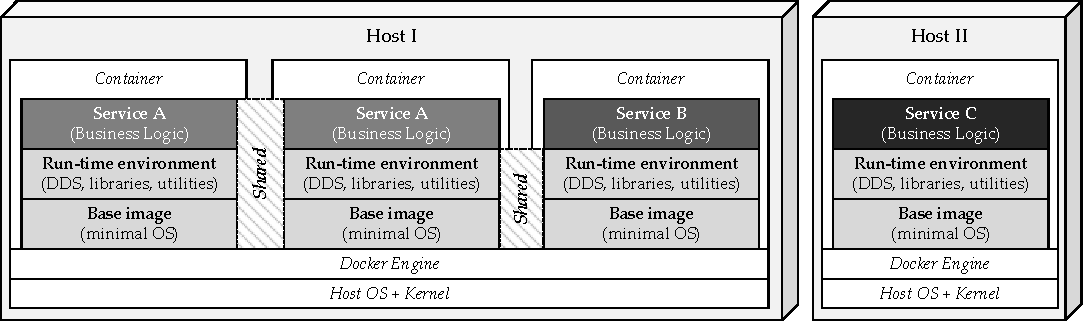
\includegraphics[width=\textwidth]{figures/docker-sharing}
  \caption[An example of containerized services]{An example of four containerized service instances, some sharing common logic to save disk space and facilitate fast updates}\label{fig:service-containers} 
\end{figure}

\autoref{fig:service-containers} shows an example of three containerized services running on two different machines, \experim{Host I} and \experim{Host II}. The former hosts two instances of \experim{Service A}, and one instance of \experim{Service B}. On the second host only one service instance is running, namely one of type \experim{Service C}. All services are packaged in their own, separate container. The containers are made up of three stacked images---the bottom two are common to all services. The bottommost image ("\emph{base image}") contains the file system layers of a minimal operating system. In the example  \emph{Debian}\footnote{\url{www.debian.org}} was used. The base image only contains a limited selection of Linux tools, such as \texttt{ls}, \texttt{cat}, etc. The purpose of a base image is to lay a good foundation that enables users to work comfortably within the container. In the case of Debian, the \emph{aptitude} package manager is additionally included which enables users to easily install further \todo{QEMU?} tools. 

Next, an \emph{intermediate image} is built on top of the base image. The intermediate image adds further layers containing the \emph{run-time environment}, and in particular, the shared libraries of OpenDDS. At this stage, the container is able to run any DDS application that was built utilizing OpenDDS. The intermediate image could theoretically contain more libraries and tools that are common to all services. In this case, however, DDS was sufficient\todo{updaten, falls es zu case study kommt} . The bottom two layers are common to all services, and thanks to \docker 's layered images, can be shared... \todo{besser erklaeren}

At the top, finally, sit the \emph{service images}. In these images the actual service logic is contained, and more precisely, the service's binary and configuration files. The service images are unique to each service, and are not shared, except when the same service is instantiated multiple times on the same machine (\experim{Service A}).



\section{Container Networking with \wnet}
\wnet\ is an open source project\footnote{\url{www.github.com/weaveworks/weave}} which is developed by a global team, mostly employed by the London-based software company \emph{Weaveworks}\footnote{\url{www.weave.works}}. The purpose of \wnet\ is to provide advanced overlay networking capabilities for \docker\ containers. As such, is designed to make up for the shortcomings of \docker 's built-in overlay networks, and more specifically, their lack of encryption and multicast support. By means of \weave\ overlay networks, dispersed containers deployed on physically isolated hosts around the world, may communicate as if they were connected via LAN. From a containerized applications' viewpoint, it does not matter whether its peers are located on the same host or within a data center on the other side of the world. 

\paragraph{}

\wnet\ is implemented as client software which is installed on each machine that partakes in the overlay. The software can be started using a single command, and in the following, all containers launched on that host will automatically connected to the overlay network. This is achieved by means of a \emph{\docker\ API proxy}. The proxy sits between \docker 's command-line client and the \docker\ daemon and intercepts all communication between the two. When the \docker\ engine is instructed to start a container, the proxy takes all precautions needed to enable overlay networking for that container. Once the connection is established, all container traffic is routed through three dedicated network channels: one TCP connection to exchange meta data about the network, and two UDP channels for duplex data exchange.

\begin{figure}[htpb]
  \centering
  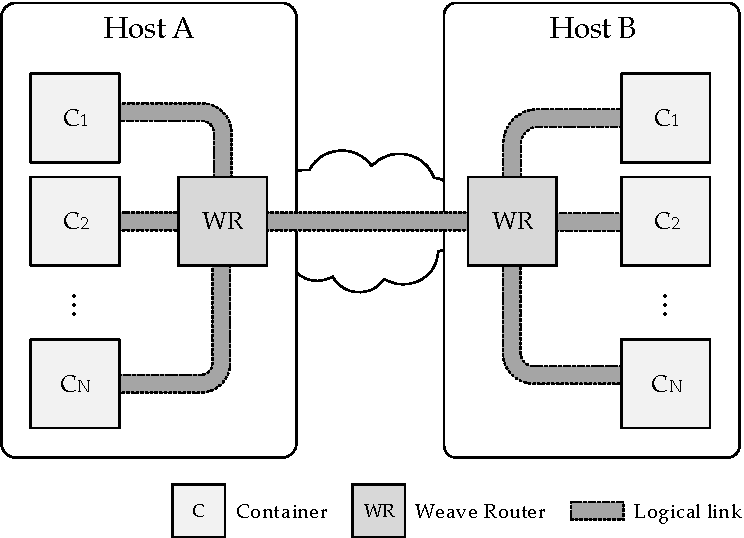
\includegraphics[width=0.7\textwidth]{figures/weave.pdf}
  \caption[An example of containers connected via \wnet\ overlay network]{A number of dispersed containers connected by a \wnet\ overlay network}\label{fig:weavescheme} 
\end{figure}

When the \weave\ software is started, a central component of \wnet , the \emph{\weave\ router} is launched (\cf\ \autoref{fig:weavescheme}). Similar to a hardware router, the \weave\ router is responsible for the forwarding and routing of data packets to their appropriate receivers. \weave\ routers can be seen as gateways through which all containers participating in a \weave\ network are connected. To facilitate routing on the data plane, a custom UDP encapsulation protocol, called \emph{sleeve}, was devised. A \weave\ router in itself is an containerized application running at all times, in the same way a daemon would. There is one of such router containers running on every host in a \weave -enabled infrastructure.

\todo[inline]{ÜBERARBEITEN}

The \weave\ router is a user space process. As such, a context switch is needed every time it is tasked to process a packet. This comes with a substantial performance overhead. Hence, as a faster alternative, the so-called \emph{fast datapath} mode was added. In this mode, packets are processed by the Linux kernel instead of by the \weave\ router. This way, the context switch into user space is omitted. \wnet\ leverages the Linux kernel's \emph{Open vSwitch datapath} module \cite{pfaff2015design} to achieve this behavior. Open vSwitch can be used to create a virtual, software-based network switch. That way, the kernel can be instructed to process packets in a certain way. For instance, the kernel can be commanded to add a VXLAN header to each packet, thereby achieving the same result as the \weave\ router, but faster. However, fast datapath mode can only be used when the underlying infrastructure allows it. The Internet is a particular example of a network where fast datapath communication is hard to achieve.


\subsection{Topology Management} 
\weave 's topology management is self-governing and self-healing. Peers continually exchange topology information and monitor the state of the network. Whenever peers lose connectivity, they continuously try to re-establish the connection until it is restored. All participating peers know the topology of the entire network. For this, \wnet\ employs a sophisticated discovery and topology management mechanism by which changes in the network topology are rapidly propagated within the network. The topology management protocol is based on a spanning-tree broadcast mechanism known from hardware switches. To further ensure that all peers have an up-to-date neighbor list at all times, \wnet\ additionally employs a custom neighbor gossiping protocol by which each peer sends update messages to a random subset of their neighbors. Updates of the network's topology are performed periodically as well as when certain events occur, such as when a node joins or leaves the network.

In order to add a new host to the overlay, the \weave\ software needs to be started on that host, referencing at least one other host in the network by its IP address. The information that a new host was added is then propagated to the other hosts in the overlay. After a short period, all hosts know that the new host was added and that a path to that host exists.

\subsection{Encryption} 
As mentioned earlier, a salient feature of \wnet\ is the ability to encrypt all traffic within the overlay network\footnote{Encryption applies end-to-end between \weave\ routers}. This is especially important for networks that span over insecure underlays, such as the Internet. To set up encryption, a shared secret (password) needs to be provided when the \weave\ router is launched. The shared secret must therefore be present on all participating hosts. From the password, salted, ephemeral session keys are generated which are then used to encrypt the network packets' payload. For each connection between any two peers, one unique session key exists.

The way encryption is applied differs depending on the forwarding mode used (sleeve or fast datapath). In fast datapath mode, a IPsec-based protocol is used, whereby each packet is wrapped in an encapsulated security payload (ESP). Because each packet in this mode is processed by the Linux kernel, encryption is applied by means of the standard Linux Kernel Crypto API which is thoroughly tested, and generally considered secure. For sleeve mode, a custom encryption algorithm based on TLS\footnote{``Transport Layer Security''} is used. As with fast datapath encryption, sleeve mode encryption utilizes shared, ephemeral session keys for each connection.

\begin{figure}[htpb]
  \centering
  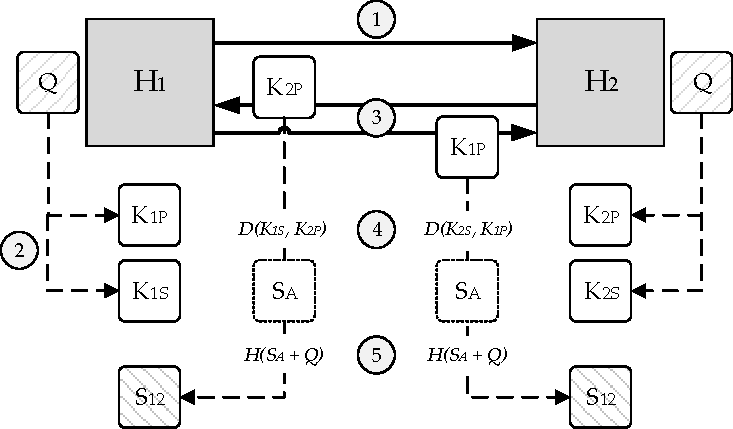
\includegraphics[width=0.6\textwidth]{figures/weave-encryption.pdf}
  \caption[\weave 's key exchange protocol]{\wnet 's key exchange protocol in sleeve mode}\label{fig:weaveencryption}
\end{figure} 
\autoref{fig:weaveencryption} depicts how these session keys are generated. In the image, two hosts ($H_1$, $H_2$) are to establish an encrypted connection. First, $H_1$ initiates the key exchange by sending a handshake message to $H_2$ \circled{1}. Then, both hosts generate their own, individual key pairs so that each host has a public key and a private key \circled{2}. The key pair for $H_1$ is $(K_{1P}, K_{1S})$ and the key pair for $H_2$ is $(K_{2P}, K_{2S})$. Once that is done, both hosts exchange their respective public keys, $K_{1P}$, and $K_{2P}$ \circled{3}. Using the peer's public key and their own private key, both hosts derive an auxiliary shared key, $S_A$, by means of Diffie--Hellman key exchange \cite{bresson2001provably}: $D(K_{1S},K_{2P})$ \circled{4}. Finally, the actual shared key can be generated. For this, both hosts append the password ($P$) to $S_A$ to provide authenticity. In order to bring the key to the desired length of 256 bit, the compounded key is additionally hashed via SHA256: $H(S_A, P)$ \circled{5}. The end result of this procedure is the final shared key, $S_{12}$, which is then used to encrypt the traffic between the two hosts.
%
%
%
%
%
%
%
%
%
%
%
%
%
%
%
%
%
%
%
%








